% *******************************************************************************
% * Copyright (c) 2007 by Elexis
% * All rights reserved. This document and the accompanying materials
% * are made available under the terms of the Eclipse Public License v1.0
% * which accompanies this distribution, and is available at
% * http://www.eclipse.org/legal/epl-v10.html
% *
% * Contributors:
% *    G. Weirich - initial implementation
% *
% *  $Id: mitmachen.tex 6282 2010-04-19 19:24:51Z niklausgiger $
% *******************************************************************************
% !Mode:: "TeX:UTF-8" (encoding info for WinEdt)
%
% Dieses Dokument behandelt die Möglichkeiten, an Elexis mitzuwirken

\chapter{Grundlagen}
\section{Einführung}
In diesem Teil des Handbuchs gehen wir auf die verschiedenen Möglichkeiten ein,
sich an Elexis zu beteiligen. Da hierfür zum Teil auch bestimmte Werkzeuge
erforderlich sind, sind einige Abschnitte eher technisch gehalten. Lassen Sie
sich davon nicht abschrecken; erstens sieht vieles komplizierter aus, als es
dann ist, und zweitens sind wir Ihnen gerne beim Einstieg behilflich.
\section{Eclipse}
\label{Eclipse}
Eclipse (\href{http://www.eclipse.org}{www.eclipse.org}) \index{Eclipse} ist die
geeignete Entwicklungsumgebung für Elexis, da Elexis selber ja eine
Eclipse-Anwendung ist.
Eclipse ist ein sehr mächtiges Werkzeug, das nicht nur zum Programmieren,
sondern auch zum Schreiben der Dokumentation etc. verwendet werden kann. Eclipse
kann für Windows, Linux, Mac und andere Betriebssysteme kostenlos heruntergeladen
werden. Sie benötigen die Variante \glqq Eclipse SDK\grqq{} für Ihr
Betriebssystem. Die Installation ist trivial: Es genügt, die heruntergeladene
Archivdatei irgendwo zu entpacken.
\section{Versionskontrollsystem}
Die Quellen, also das, woraus das Gesamtprojekt \textit{elexis} letztlich
hergestellt wird, befinden sich in einem Versionskontrollsystem
\index{Versionskontrollsystem} bzw.
\glqq revision control system\grqq. \index{RCS}Ein Versionskontrollsystem ist ein
Ablagesystem, das Dateien aller Art in einem speziellen Speicher, einem \glqq
Repository\grqq \index{Repository}aufbewahren kann. Das besondere daran sind zwei Dinge:
\begin{itemize}
\item Es werden sämtliche Versionen jeder Datei aufbewahrt und mit Datum und
Ersteller markiert. Man kann zu jedem Zeitpunkt zu jeder beliebigen Version
einer Datei zurückkehren. Neue Versionen werden automatisch jedesmal erzeugt,
wenn eine Datei verändert wurde.
\item Wenn verschiedene Personen gleichzeitig Änderungen an einer Datei machen,
dann werden diese Änderungen wenn immer möglich automatisch zusammengeführt.
Dies gelingt nur dann nicht, wenn zufällig mehrere Leute genau dieselbe Stelle
einer Datei bearbeitet haben. In diesem Fall markiert das Versionskontrollsystem
diese Stelle als Konflikt, der später manuell aufgelöst werden muss.
\end{itemize}

Das Versionskontrollsystem, das wir bei Elexis benutzen, ist das relativ neue \glqq
Sub\-ver\-sion\grqq (\href{http://subversion.tigris.org}{subversion.tigris.org}). \index{Subversion}
Das Repository befindet sich auf einem Server des OpenSource Hosters
\href{http://www.sourceforge.net}{Sourceforge} (\glqq Quellenschmiede\grqq).

Da Elexis ein OpenSource-System ist, ist der Lesezugriff auf das Repository
unbeschränkt frei. Es ist also ohne weiteres jedem möglich die Quellen auf den
eigenen Computer herunterzuladen, und dort eine eigene Version von Elexis
herzustellen.

Um das Projekt vor Vandalismus zu schützen, kann allerdings der
\textit{Schreibzugriff} nicht unkontrolliert freigegeben werden. Änderungen am
Quelltext können zwar von jedem gemacht werden, aber nicht jeder kann eigene
Änderungen ins Repository hochladen. Wir werden in aller Regel aber jedem, der
ernsthaftes Interesse zeigt, Schreibzugriff gewähren.

\section{Benötigte Hilfsmittel}
Um auf die Dateien im Repository zugreifen zu können, benötigen Sie einen
\textit{Subversion Client}. Dies kann je nach Ihrer Arbeitsumgebung ein
integrierter Client, beispielsweise für Eclipse sein, oder ein
Kommandozeilenclient. Hier beschreiben wir die Einrichtung des integrierten
Subversion clients für Eclipse, welcher als \textit{Plugin} für Eclipse
bezogen werden kann.
\subsection{Einrichtung des Subclipse-Clients in Eclipse}
\label{subclipse}\index{Subversion!Plugin für Eclipse}
\begin{itemize}
  \item Wählen Sie in Eclipse das Menu \textsc{Help -- Software~Updates -- Find
  and install}
  \item Wählen Sie dann den Punkt \textit{Search for new features to install} und
  klicken Sie auf \textsc{Next}
  \item Klicken Sie \textsc{New Remote Site}
  \item Geben Sie für \glq Name\grq ein: Sub\-clipse und für \glq URL\grq:
  http://subclipse.tigris.org/update\_1.2.x
  \item Wählen Sie bei \glqq Select features to install\grqq Subclipse aus und
  klicken Sie auf \textsc{Next}. Nachdem Sie den Lizenzbedingungen zugestimmt
  haben, wird Subclipse installiert,

\end{itemize}
\subsection{Subversion Kommandozeilen-Client}
\label{subversionclient}\index{Subversion!Kommandozeilen-Client}
Selbstverständlich können Sie auf das Subversion-Repository auch zugreifen. ohne
zuvor Eclipse installieren zu müssen. Vielleicht möchten Sie doch lieber mit
einer anderen Entwicklungsumgebung arbeiten, oder vielleicht möchten Sie nur die
Dokumentations-Quellen holen, um mit einem anderen \TeX-Werkzeug damit zu
arbeiten. In diesen Fällen benötigen Sie einen Kommandozeilen-Client für
Subversion. Sie können diesen bei
\href{http://subversion.tigris.org}{subversion.tigris.org} für Ihr
Betriebssystem herunterladen.

\section{erstes Herunterladen der Quellen}
\subsection{Mit Eclipse}
Öffnen Sie in Eclipse die Subversion-Perspektive (\textsc{Window -- Open
Perspective -- Other -- SVN Repository Exploring}). Klicken Sie mit der rechten
Maustaste ins Fenster \glqq SVN Repository\grqq{} und wählen Sie \textsc{New --
Repository Location}. Geben Sie als URL ein:
\begin{quote}https://elexis.svn.sourceforge.net/svnroot/ch.elexis/trunk\end{quote}. Wenn alles stimmt, erscheint
jetzt ein Repository-Symbol mit diesem Namen im Fenster. Klicken Sie auf das
Plus-Zeichen links und Sie sehen alle Unterprojekte, aus denen Elexis besteht.
Wählen Sie eins oder mehrere der interessierenden Projekte aus, klicken Sie mit
der rechten Maustaste und wählen Sie \textsc{checkout}. Dieser Prozess dauert
einige Zeit, in der \glqq nichts\grqq{} zu passieren scheint (kann mehrere Minuten
bis zu einer viertel Stunde dauern). Bleiben Sie bei allen Rückfragen immer
bei den Voreinstellungen und klicken Sie \textsc{Next} bzw. \textsc{finish}.
\subsection{Mit dem Kommandozeilenclient}
Öffnen Sie in dem Ordner, in dem Sie Ihr Elexis-Projekt unterbringen wollen,
eine Kommandozeile und geben Sie dort ein: \begin{quote}svn checkout
https://elexis.svn.sourceforge.net/svnroot/ch.elexis/trunk\end{quote} Dies würde das gesamte Projekt
herunterladen. Wenn Sie nur ein einzelnes Unterprojekt, beispielsweise die
Dokumentation beziehen wollen, dann können Sie eingeben: \begin{quote}svn checkout
https://elexis.svn.sourceforge.net/svnroot/ch.elexis/trunk/dokumentation\end{quote} Für weitere
Möglichkeiten konsultieren Sie bitte die ausgezeichnete Dokumentation zu
Subversion.

\section{Arbeiten mit den Quellen}
Das oben beschriebene \glqq checkout\grqq{} ist nur beim ersten Herunterladen des
Projektes notwendig. Später starten Sie jeden Arbeitszyklus mit einem \glqq
update\grqq, bearbeiten die Quellen, und führen am Schluss ein \glqq commit\grqq{}
durch (sofern Sie die entsprechenden Rechte\footnote{Um Commitrechte zu
bekommen, müssen Sie jemanden von den Projektadministratoren fragen, und Sie
müssen einen Account bei Sourceforge haben} haben)
\subsection{update}
\begin{itemize}
  \item in Eclipse: Rechts-Klick auf das Projekt und \textsc{Team-Update}
  wählen.
  \item Kommandozeile: Ins Projektverzeichnis wechseln und \textsc{svn update}
  eingeben. Dies holt alle Änderungen, die in der Zwischenzeit vielleicht von
  anderen gemacht worden sind, auf Ihren Computer
\end{itemize}
\subsection{commit}
\begin{itemize}
  \item in Eclipse: Rechts-Klick auf das Project und \textsc{Team-Commit}
  wählen.
  \item Kommandozeile: Ins Projektverzeichnis gehe und \textsc{svn commit
  -m\glqq Beschreibung Ihres commits\grqq} eingeben. Dies schreibt Ihre Änderungen
  ins Repository zurück und markiert sie mit der gegebenen Beschreibung.
\end{itemize}


\chapter{Programmieren}
\section{Wer kann mitmachen?}
\begin{itemize}
  \item Wer Java und SWT beherrscht oder es lernen möchte
  \item Wer das Elexis Kernsystem verbessern oder ausbauen möchte
  \item Wer eigene Plugins für bestimmte Funktionalitäten entwickeln möchte
\end{itemize}
\section{Wie kann man mitmachen}
Wir empfehlen unbedingt Eclipse als Ent\-wick\-lungs\-platt\-form. Man kann an Ele\-xis
natür\-lich auch mit anderen IDE's arbeiten, aber vieles wird dann schwieriger.
Folgen Sie dem oben (s. \pageref{Eclipse})) beschriebenen Vorgehen, um Eclipse
und das Subclipse-Plugin zu installieren.

Da das Thema \glqq Programmieren an Elexis\grqq{} deb Rahmen dieses Handbuchs
sprengen würde, möchten wir für weitere Informationen hierzu auf die Website des
Elexis-Projekts, Abschnitt \glqq Developers\grqq{}verweisen.

\chapter{Testen}
\section{Wer kann mitmachen}
Hierfür sind wir in erster Linie an Leuten interessiert, die Elexis \glqq
echt\grqq{} einsetzen wollen, und die bereit sind, die zusätzliche Zeit
aufzuwenden, die nötig ist, um etwaige Fehler oder Ungereimtheiten möglichst
aussagekräftig und nachvollziehbar an uns zurückzumelden.
\section{Wie kann man mitmachen}
\label{senderrors}
Dazu benötigen Sie im Grunde nur eine der Basisinstallationen. Wichtig ist, dass
Sie den Abschnitt \glqq E-Mail\grqq{} unter \textsc{Datei -- Einstellungen}
korrekt ausfüllen (s. fig. \ref{fig:mailsettings})
\begin{figure}[htp]
\begin{center}
  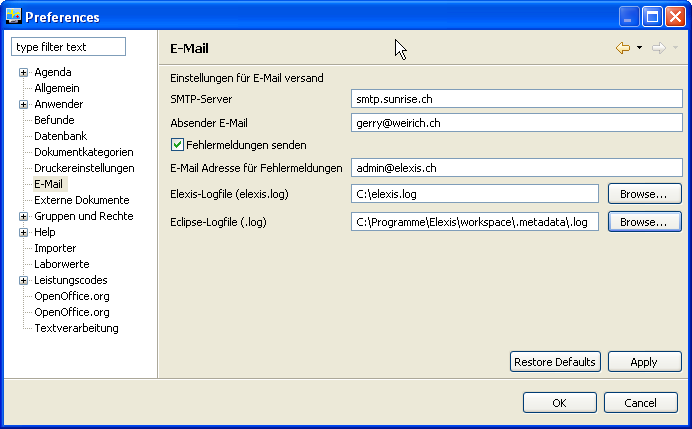
\includegraphics[width=150mm]{images/mailsettings}
  \caption{Einstellungen für Fehlermeldungen}
  \label{fig:mailsettings}
\end{center}
\end{figure}
\section{Vorgehen bei Auftreten eines Fehlers}

Keine Software kann von vornherein garantiert fehlerfrei sein. Das gilt für
ClosedSource ebenso wie für OpenSource-Programme. Bei letzteren ist allerdings
eine offene Fehlerkultur üblich, die es erlaubt, allfällige Fehler möglichst
rasch und korrekt zu beheben.
\subsection{Welche Fehler soll man melden}
Wir sind der Ansicht, dass der Begriff \glqq Fehler\grqq{} nicht besonders eng
gefasst sein muss. Wenn Sie der Meinung sind, dass irgendein Verhalten des
Programm nicht so ist, wie es sein sollte, dann halten wir das für meldenswert.
\subsection{Einfache Rückmeldung}
Wenn ein Fehler oder ein \glqq unklares Verhalten\grqq{}des Programms auftritt,
dann versuchen Sie als erstes, das Phänomen zu reproduzieren. Wählen Sie dann
das Menu \textsc{Hilfe -- Fehlermeldung senden}. Beschreiben Sie im darauf
öffnenden Dialog möglichst genau die Schritte, mit denen der Fehler
hervorgerufen wurde resp. reproduziert werden kann. Sie erzeugen damit eine
Mail, welche nebst Ihrer Meldung auch zwei Logdateien an uns sendet. Diese
enthalten keine persönlichen oder vertraulichen Inhalte (Sie können sie
jederzeit mit einem einfachen Texteditor ansehen), sondern nur Informationen
über Programminterna zum gegebenen Zeitpunkt.
\subsection{Veröffentlichung von Fehlern}
Wenn Sie der Meinung sind, dass der von Ihnen entdeckte Fehler von grösserer
Bedeutung ist, dann können Sie einen Eintrag für diesen Fehler direkt im
Bug-Tracker von Sourceforge machen.
\section{Vorgehen bei Wunsch nach Programmfeatures}

\chapter{Übersetzen}
Elexis ist im Grunde polyglott angelegt. Die meisten Texte können relativ leicht
und ohne Programmierkenntnisse gegen ihre Äquivalente in anderen Sprachen
ausgetauscht werden. Allerdings könnte -- wie so oft -- der Teufel unerkannt im
Detail stecken. Mangels Erfahrung können wir nicht sagen, ob Elexis in einer
anderen Sprache als deutsch tatsächlich reibungslos funktionieren würde. Am
weitesten sind die Bemühungen in Französisch fortgeschritten\footnote{Mit
besonderem Dank an Dominique Bünzli von
\href{http://www.medclipse.ch}{www.medclipse.ch}, der bereits ca. 1/3 der Texte
von Elexis auf französisch übersetzt hat.}.
Vom Kern-Team selbst gibt es bisher keine Übersetzungsbemühungen, da andere
Arbeiten höher priorisiert sind. Wir werden aber jede(n) der/die Bereitschaft
signalisiert, Übersetzungsarbeiten zu machen, nach Kräften unterstützen. Es sei
nochmals darauf hingewiesen, dass hierfür keine Programmierkenntnisse
erforderlich sind.

\chapter{Dokumentation}
\section{Wer kann mitmachen?}
\label{dokumentation}
Kurze Antwort: Jeder, der sich an der Dokumentation von Elexis beteiligen
möchte, ist herzlich willkommen. Benötigt werden Dokumentationskapitel,
Kurzanleitungen, Erfahrungsberichte und Anderes.

\section{Wie kann man mitmachen?}
\subsection{Einzelne Artikel}
Senden Sie Ihren Artikel einfach an dokumentation@elexis.ch
\subsection{Stärkeres Engagement}
Wenn Sie Artikel korrigieren, oder mehrere Dokumentationselemente einbringen
wollen, ist es einfacher, Sie arbeiten direkt an den Quelltexten der
Dokumentation.
\subsubsection{Quelltext und Vorbedingungen:}
Die Elexis-Dokumentation basiert auf \TeX - Quelltexten. Es genügt daher im
Prinzip ein einfacher Texteditor, um die Quellen zu bearbeiten. Komfortabler ist
es aber natürlich, wenn Sie eine \LaTeX - Entwicklungsumgebung haben. Für Windows
ist beispielsweise MiKTeX \href{http://www.miktex.org}{www.miktex.org}
empfehlenswert. Unter Mac möchten Sie vielleicht MacTex
(\href{http://www.tug.org/mactex}{www.tug.org/mactex}) verwenden, unter Linux
ist teTex die Standard-Basis, welche bei fast allen Distributionen dabei ist
(aber vielleicht separat installiert werden muss). Eine sehr komfortable
Entwicklungsumgebung unter Linux mit KDE-Oberfläche ist kile
\href{http://kile.sourceforge.net/}{kile.sourceforge.net}. Auch dieses ist bei
vielen Distributionen bereits eingeschlossen und kann deswegen mit dem
Softwareverwaltungstool der Distribution komfortabel installiert werden.

\subsection{Regeln}
Damit die gemeinsame Arbeit an den Quelltexten nicht zu unnötigen Reibereien und
Ärger führt, sollten einige Regeln beachtet werden:
\begin{itemize}
  \item Eigene Texte sollen möglichst umgehend hochgeladen werden, damit alle
  immer auf dem aktuellen Stand sein können.
  \item Ein hochgeladener Text braucht nicht fertig und auch nicht stilistisch
  perfekt zu sein, aber er sollte fehlerfrei mit latex und PDFLaTeX compiliert
  werden können. Beachten Sie bitte diese Grundregel, die analog auch für die
  Java-Programmierer gilt: Was im Repository ist, braucht weder fehlerlos noch
  perfekt zu sein, aber es \textbf{muss} compilierbar sein, damit andere nicht
  unnötig Zeit mit Fehlersuche vergeuden müssen.
  \item Fremde Texte sollen nur sehr sparsam korrigiert werden. Verschiedene
  Leute schreiben mit verschiedenem Stil und das ist auch gut so. Bitte keine
  Stilkorrekturen machen. Wenn Sie auf einen sachlichen oder Ihrer Meinung nach
  klaren stilistischen Fehler stossen, sollten Sie den Autor fragen, ob Sie es
  ändern dürfen.
  \item Reine Orthographiefehler hingegen dürfen auch in fremden Texten
  jederzeit korrigiert werden.
  \item Eigene und fremde Texte dürfen nachträglich auch von anderen ergänzt
  werden.
\end{itemize}

\chapter{Entwicklung fördern}
Sie möchten eine bestimmte Funktion oder eine bestimmte Erweiterung in Elexis?
Sie haben Bedarf für Statistik- oder Controlling-Funktionen? Im Prinzip: Kein
Problem. Elexis ist offen genug, dass all dies und mehr nachträglich
programmiert werden kann. Sie können:
\begin{itemize}
  \item Einen Java-Programmierer engagieren, der die gewünschte Funktion zu
  beliebig auszuhandelnden Bedingungen für Sie programmiert.
  \item Uns genau erklären, was Sie wollen; wir werden Ihnen dann einen
  verbindlichen Voranschlag machen, wieviel es Sie kosten wird und wie
  lange die Entwicklung maximal dauern wird. Ausserdem stellen wir die
  Bedingung, dass wir das in Ihrem Auftrag programmierte Element nicht nur
  Ihnen, sondern allen Elexis-Anwendern zur Verfügung stellen dürfen.
\end{itemize}
